% -- Encoding UTF-8 without BOM
% -- XeLaTeX => PDF (BIBER)

\documentclass[french]{cv-style}      % Add 'print' as an option into the square bracket to remove colours from this template for printing.
                                      % Add 'espanol' as an option into the square bracket to change the date format of the Last Updated Text
                                      % Add 'french' as an option into the square bracket to change the date format of the Last Updated Text

% \sethyphenation[variant=british]{english}{} % Add words between the {} to avoid them to be cut
\sethyphenation{french}{} % Add words between the {} to avoid them to be cut

\cvheadheight{3.5cm}
\cvasidewidth{4.7}
\cvasidevpos{3.5}
\cvmainwidth{11.5cm}
\geometry{a4paper, left=6.4cm, top=2.5cm, right=1cm, bottom=1cm, nohead, nofoot}

\usepackage[sectcntreset]{bibtopic}
\usepackage{natbib}
\bibliographystyle{bib/achemso_perso}
\AtBeginDocument{\nocite{achemso-control}}

\usepackage{hyperref}

\begin{document}

\header{Germain }{Salvato Vallverdu}{Maître de conférences -- Docteur en Chimie-Physique}          % Your name
\lastupdated

%----------------------------------------------------------------------------------------
%	SIDEBAR SECTION  -- In the aside, each new line forces a line break
%----------------------------------------------------------------------------------------

\begin{aside}
    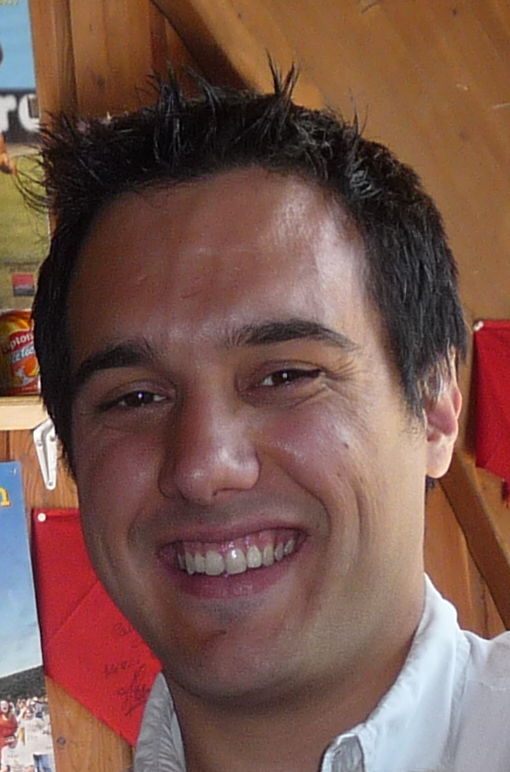
\includegraphics[width=.9\columnwidth]{img/germain}
    10 août 1983, France
    Marié, 2 enfants
    %
    \section{Contact}
    germain.vallverdu@univ-pau.fr
    ~
    05 59 40 78 51
    06 88 59 08 87
    ~
    IPREM
    Technopôle Hélioparc
    2 ave du Président P. Angot
    64053 Pau cedex 9
    %
    \section{Chimie Théorique}
    Modélisation
    Développement
    Stratégie de calculs
    VASP, CRYSTAL (solide)
    Gaussian (molécule)
    DL-POLY, AMBER (dynamique)
    %
    \section{Programmation}
    Fortran, C
    Python
    \LaTeX{}, HTML/CSS
    %
    ~
    \section{Langues}
    Français
    Anglais (Professional)
    %
    \section{Sur internet}
    \href{http://orcid.org/0000-0003-1116-8776}{$\vcenter{\hbox{
\includegraphics{img/iD-icon}}}$ orcid.org/0000-0003-1116-8776}
    \href{https://github.com/gVallverdu}{$\vcenter{\hbox{
\includegraphics[height=16pt]{img/GitHub-Mark}}}$ gVallverdu}
    %
\end{aside}

\section{Résumé}

Physico-chimiste de formation, je suis Maître de conférences à l'Université de
Pau et des Pays de l'Adour dans l'Institut des sciences analytiques et de
physico-chimie pour l'environnement et les matériaux (IPREM). Mes activités de
recherche concernent le développement de stratégies calculatoires pour l'étude
de systèmes complexes par des méthodes de chimie théorique à différentes échelles
de temps et ou d'espace. J'effectuer mes enseignement à l'UFR des sciences et
techniques de Pau.

%----------------------------------------------------------------------------------------
%	SKILLS SECTION
%----------------------------------------------------------------------------------------

%\section{skills}
%  \vspace{-0.2cm}

%Skill 1, skill 2, skill 3, skill 4, skill 5.

%----------------------------------------------------------------------------------------
%	WORK EXPERIENCE SECTION
%----------------------------------------------------------------------------------------

\section{Experience Professionnelle}

\begin{entrylist}
%------------------------------------------------
\entry
  {depuis 2010~}
  {Université de Pau et des Pays de l'Adour}
  {Pau, France}
  {\jobtitle{Maître de conférences}\\
   Chimie théorique et simulation numérique.
   Surface, interface et réactivité.}
%------------------------------------------------
\entry
  {2009--2010}
  {CEA - DAM}
  {Bruyères le châtel, France}
  {
  %\jobtitle{Postdoctoral position}\\
  \jobtitle{Chercheur-ingénieur}\\
  %Development and implementation of mesoscopic models for reactive shock waves propagation in heterogeneous systems.\\
  Développement et implémentation d'un modèle mésoscopique pour l'étude de la propagation
  d'ondes de chock réactives dans un système hétérogène.
%  Detailed achievements:
%  \begin{itemize}
%    \item Achievement 1. Achievement 1. Achievement 1.
%    \item Achievement 2. Achievement 2. Achievement 2. Achievement 2. Achievement 2. Achievement 2.
%    \item Achievement 3. Achievement 3. Achievement 3. Achievement 3.
%  \end{itemize}
  }
%------------------------------------------------
\entry
  {2006--2009}
  {Université Paris-Sud 11}
  {Orsay, France}
  {
  %\jobtitle{PhD Student}\\
  \jobtitle{Allocataire de recherche, moniteur}\\
  %Theoretical study of photophysical processes in fluorescent proteins.\\
  Étude théorique de processus photophysiques dans les protéines fluorescentes.
%  Detailed achievements:
%  \begin{itemize}
%    \item Achievement 1. Achievement 1. Achievement 1. Achievement 1. Achievement 1. Achievement 1. Achievement 1. Achievement 1.
%  \end{itemize}
  }
%------------------------------------------------
\end{entrylist}

%----------------------------------------------------------------------------------------
%	EDUCATION SECTION
%----------------------------------------------------------------------------------------

\section{Formation}

\begin{entrylist}
%------------------------------------------------
\entry
{2006-2009}
{Doctorat de chimie {\normalfont spécialité chimie-théorique}}
{Université Paris-Sud 11}
{Mention très honorable}
%------------------------------------------------
\entry
{2004-2006}
{Master de chimie {\normalfont spécialité physico-chimie moléculaire}}
{Université Paris-Sud 11}
{Mention TB}
%------------------------------------------------
\entry
{2003-2004}
{Licence de chimie-physique}
{Université Paris-Sud 11}
{Mention TB}
%------------------------------------------------
\entry
{2003-2006}
{Magistère de Physico-Chimie Moléculaire}
{Université Paris-Sud 11 -- ENS Cachan}
{}
%------------------------------------------------
\entry
{2001-2003}
{CPGE {\normalfont PCSI-PC}}
{Lycée François Arago, Perpignan}
{}
\end{entrylist}

%----------------------------------------------------------------------------------------
%	OTHER QUALIFICATIONS SECTION
%----------------------------------------------------------------------------------------

\section{Publications}

\nocite{vallverdu2016, guille2015, Guille2014, Martin2012, Maillet2011, Jonasson2011, Vallverdu2010, Vallverdu2009}
\begin{btSect}{bib/articles}
    \btPrintCited
\end{btSect}

%----------------------------------------------------------------------------------------
%	AWARDS SECTION
%----------------------------------------------------------------------------------------

% \section{awards}
%
% \begin{entrylist}
% %------------------------------------------------
% \entry
% {2014}
% {Award name}
% {Institution}
% {Award description. Award description. Award description. Award description. Award description. Award description. Award description. }
% %------------------------------------------------
% \end{entrylist}

%----------------------------------------------------------------------------------------
%	INTERESTS SECTION
%----------------------------------------------------------------------------------------

% \section{interests}
%   \vspace{-0.2cm}
%
% \textbf{professional:} professional interest 1, professional interest 2 and professional interest 3.
% \textbf{personal:} personal interest 1, personal interest 2, personal interest 3 and personal interest 4.

%----------------------------------------------------------------------------------------

\end{document}
